% ============================================== %

%%%%%%%%%%%%%%%%%%%%%%%%%%%%%%%%%%%%%%%%%%%%%%%%%%
%%%			  05 Trabalho Prático 05		   %%%
%%%%%%%%%%%%%%%%%%%%%%%%%%%%%%%%%%%%%%%%%%%%%%%%%%

% ============================================== %

\section{Trabalho Prático 05}

Fazer os gráficos $F\times \delta_v$ (deslocamento vertical) e $N\times \delta_v$ para
$y \in \left[0,40; 0,20\right]$ m. Adotar:

$$
\left\{\begin{array}{lcl}
	\Delta y &=& -0,01\text{ m} \\
	EA_0 &=& 133,865\text{ kN} \\
	L &=& 4,0\text{ m} \\
	H &=& 0,20\text{ m} \\
\end{array}\right.
$$

\begin{figure}[H]
	\centering
	\caption{Sistema estrutural do Trabalho Prático 05.}
	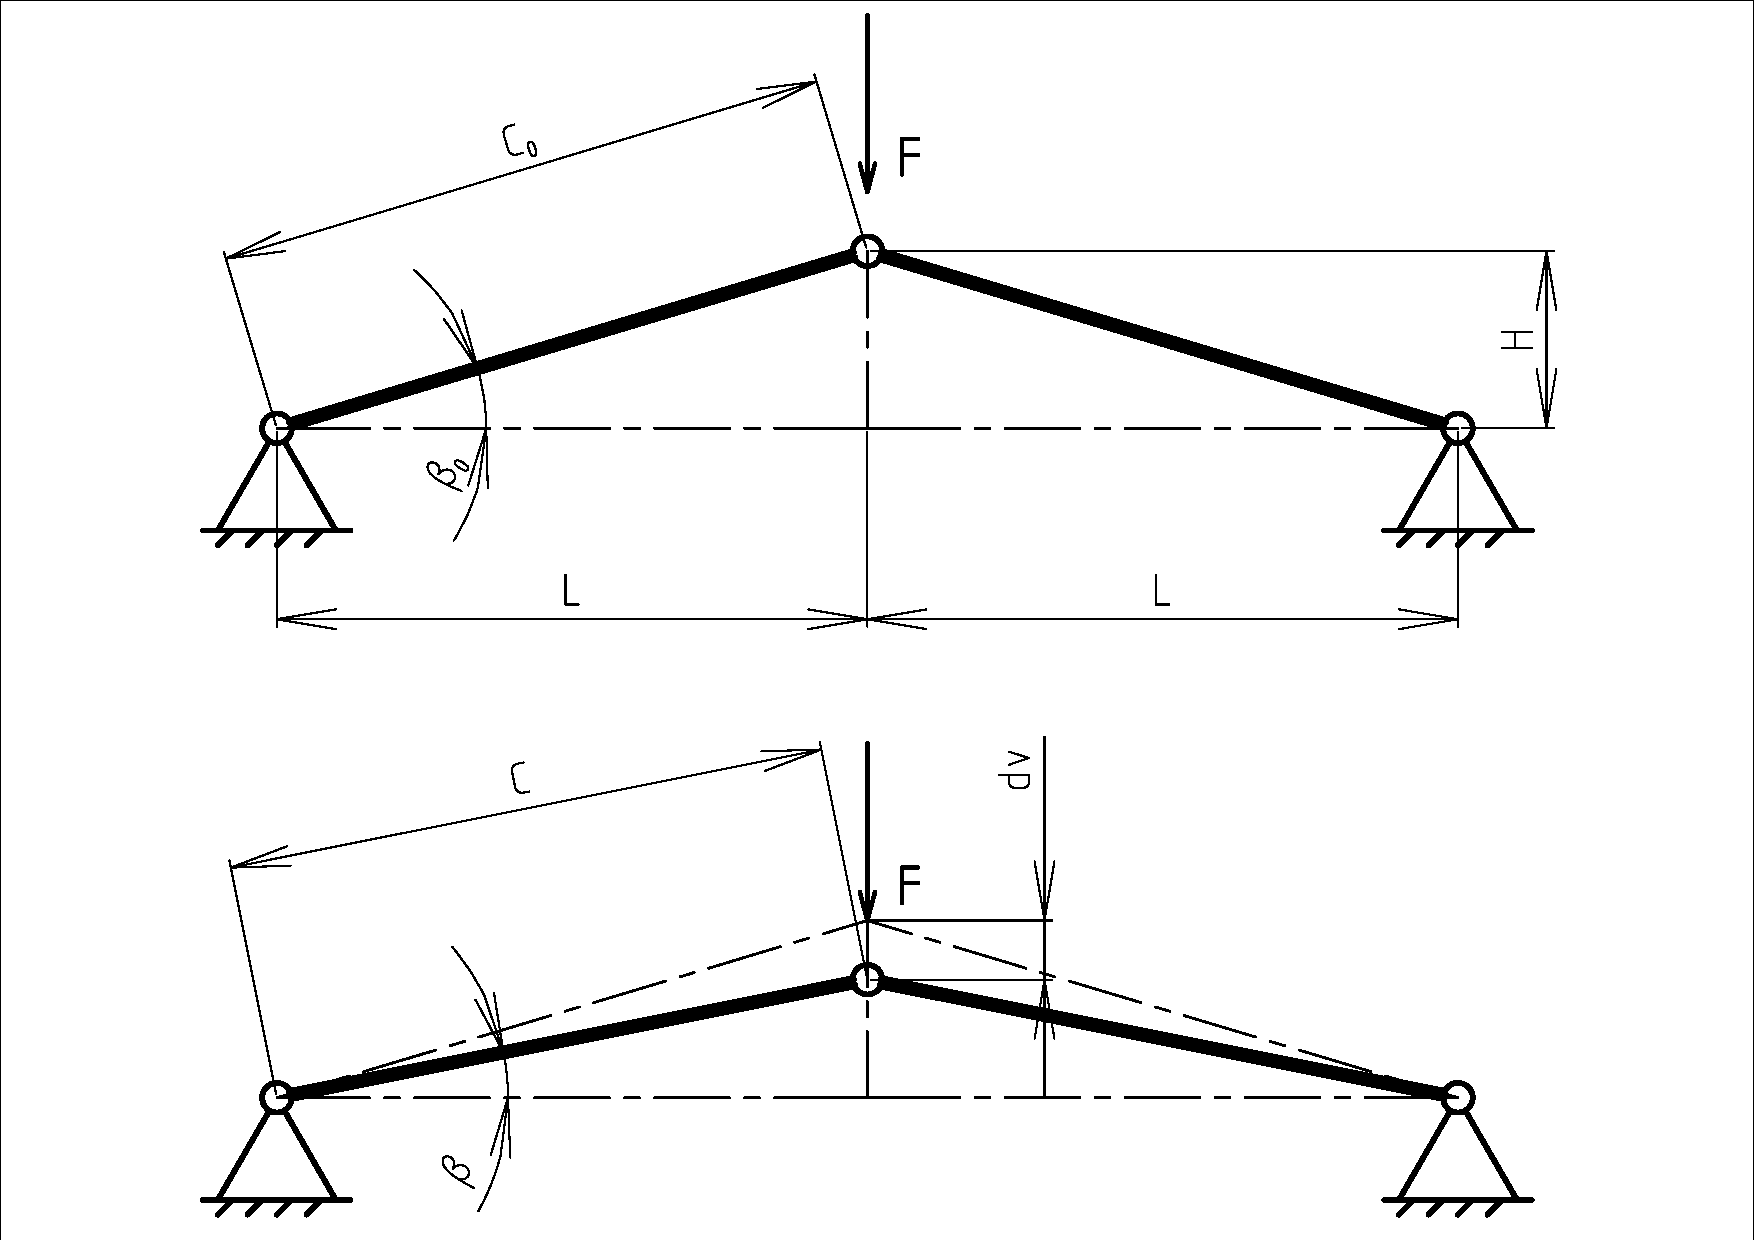
\includegraphics[
		trim=30mm 4mm 30mm 2mm,
		clip,
		width=0.75\textwidth
	]{figuras/TPs-5.pdf}
\end{figure}


% ================ Resolução TP-05 ================
\begin{textocaixa}
\hspace{10mm}




\end{textocaixa}